\chapter{\ifenglish Background Knowledge and Theory\else ทฤษฎีที่เกี่ยวข้อง\fi}


\section{ด้านโครงสร้างเว็บแอปพลิเคชัน}
ในส่วนนี้จะอธิบายถึงโครงสร้างของเว็บแอปพลิเคชันที่ใช้ในการพัฒนา

\subsection{MVC Architecture}
MVC \cite{web:codebee} เป็นตัวย่อของคำว่า Model View Controller ใช้เรียกรูปแบบการพัฒนาซอฟต์แวร์ที่มีโครงสร้างซึ่งแบ่งออกมาเป็น 3 ส่วนหลัก ตามตัวย่อของชื่อ รูปแบบการพัฒนาซอฟต์แวร์แบบ MVC ถูกนำไปใช้ในขั้นตอนการพัฒนาหลากหลายภาษา
เพราะ MVC เป็นเพียงหลักการออกแบบโปรแกรม (Design Pattern) รูปแบบหนึ่งเท่านั้น ซึ่งเป็นที่นิยมมาก
ในการนำมาพัฒนาแอพพลิเคชั่นซอฟต์แวร์แต่ละแพลตฟอร์ม และประยุกต์ใช้ในอีกหลาย ๆ ด้าน
\subsubsection{ส่วนของ Model (M)}
model คือส่วนของการเก็บรวบรวมข้อมูล ไม่ว่าข้อมูลนั้น ๆ จะถูกจัดเก็บในรูปแบบใดก็ตาม ในฐานข้อมูล
แบบเป็น Object Class หรือที่นิยมเรียกกันว่า VO ( Value Object ) หรือเก็บเป็นไฟล์ข้อมูลเลย
เมื่อข้อมูลถูกโหลดเข้ามาจากที่ต่าง ๆ และเข้ามายังส่วนของโมเดล ตัวโมเดลจะทำการจัดการตระเตรียมข้อมูลให้เป็นรูปแบบที่เหมาะสม เพื่อรอการร้องขอข้อมูลจากส่วนของ Controller
\subsubsection{ส่วนของ View (V)}
view คือส่วนของการแสดงผล หรือส่วนที่จะปฏิสัมพันธ์กับผู้ใช้งาน ( User Interface ) หน้าที่ของ view
ในการเขียนโปรแกรมแบบ MVC คือคอยรับคำสั่งจากส่วนของ Controller และ End User เริ่มแรกเลยตัววิว
อาจจะได้รับคำสั่งจาก Controller ให้แสดงผลหน้า Home และเมื่อผู้ใช้งานหน้าเว็บกดปุ่มสั่งซื้อ View จะส่งข้อมูลไปให้ Controller เพื่อประมวลผลและแสดงบางอย่างจาก Action นั้น
\subsubsection{ส่วนของ Controller (C)}
controller คือส่วนของการเริ่มทำงาน และรับคำสั่ง โดยที่คำสั่งนั้นจะเกิดขึ้นในส่วนการติดต่อกับผู้ใช้งานคือ view
เมื่อผู้ใช้งานทำการ Interactive กับ UI view จะเกิดเหตุการณ์หรือข้อมูลบางอย่างขึ้น ตัววิวจะส่งข้อมูลนั้น
มายัง controller ตัว controller จะทำการประมวลผลโดยบางคำสั่งอาจจะต้องไปติดต่อกับ model ก่อน
เพื่อทำการประมวลผลข้อมูลอย่างถูกต้องเรียบร้อยแล้วก็จะส่งไปยัง view เพื่อแสดงผลตามคำสั่งที่ end user ร้องขอมา
Controller จะทำหน้าที่เป็นตัวกลางระหว่าง Model และ View ให้ทำงานร่วมกันอย่างมีประสิทธิภาพและตรงกับ
ความต้องการของ End User มากที่สุด

\subsection{RESTful API}
RESTful API \cite{web:RESTful} เป็นอินเทอร์เฟซที่ระบบคอมพิวเตอร์สองระบบใช้เพื่อแลกเปลี่ยนข้อมูลผ่านอินเทอร์เน็ตได้อย่างปลอดภัย แอปพลิเคชันทางธุรกิจส่วนใหญ่ต้องสื่อสารกับแอปพลิเคชันภายในอื่นๆ และของบุคคลที่สามเพื่อทำงานต่างๆ ตัวอย่างเช่น หากต้องการสร้างสลิปเงินเดือน ระบบบัญชีภายในของคุณต้องแบ่งปันข้อมูลกับระบบธนาคารของลูกค้าเพื่อออกใบแจ้งหนี้และสื่อสารกับแอปพลิเคชันบันทึกเวลาปฏิบัติงานภายในโดยอัตโนมัติ RESTful API ให้การสนับสนุนการแลกเปลี่ยนข้อมูลนี้เพราะเป็นระบบที่มีมาตรฐานการสื่อสารระหว่างซอฟต์แวร์ที่ปลอดภัย เสถียร และมีประสิทธิภาพ
\subsubsection{API (Application Programming Interface)}
ส่วนต่อประสานโปรแกรมประยุกต์ (Application Programming Interface หรือ API) กำหนดกฎที่คุณต้องปฏิบัติตามเพื่อสื่อสารกับระบบซอฟต์แวร์อื่น โดยนักพัฒนาเปิดเผยหรือสร้าง API เพื่อให้แอปพลิเคชันอื่นสามารถสื่อสารกับแอปพลิเคชันของตนได้ทางโปรแกรม ตัวอย่างเช่น แอปพลิเคชันบันทึกเวลาปฏิบัติงานแสดง API ที่ขอชื่อเต็มของพนักงานและช่วงวันที่ เมื่อได้รับข้อมูลนี้แล้ว ระบบจะประมวลผลบันทึกเวลาปฏิบัติงานของพนักงานเป็นการภายใน และส่งกลับจำนวนชั่วโมงที่ทำงานในช่วงวันที่ดังกล่าว
ทั้งนี้คุณสามารถมองได้ว่า API เว็บเป็นเกตเวย์ระหว่างไคลเอ็นต์และทรัพยากรบนเว็บ

ไคลเอ็นต์
ไคลเอ็นต์คือผู้ใช้ที่ต้องการเข้าถึงข้อมูลจากเว็บ โดยไคลเอ็นต์อาจเป็นบุคคลหรือระบบซอฟต์แวร์ที่ใช้ API ก็ได้ ตัวอย่างเช่น นักพัฒนาสามารถเขียนโปรแกรมที่เข้าถึงข้อมูลสภาพอากาศจากระบบสภาพอากาศ หรือคุณสามารถเข้าถึงข้อมูลเดียวกันจากเบราว์เซอร์เมื่อคุณเยี่ยมชมเว็บไซต์รายงานสภาพอากาศได้โดยตรง

ทรัพยากร
ทรัพยากรคือข้อมูลที่แอปพลิเคชันต่างๆ มอบให้แก่ไคลเอ็นต์ โดยทรัพยากรอาจเป็นรูปภาพ วิดีโอ ข้อความ ตัวเลข หรือข้อมูลประเภทใดก็ได้ ทั้งนี้เครื่องคอมพิวเตอร์ที่มอบทรัพยากรให้แก่ไคลเอ็นต์นั้นเรียกอีกอย่างว่าเซิร์ฟเวอร์ องค์กรต่างๆ ใช้ API เพื่อแบ่งปันทรัพยากรและให้บริการเว็บในขณะที่ยังคงดูแลรักษาความปลอดภัย การควบคุม และการรับรองความถูกต้องไปพร้อมกัน นอกจากนี้ API ยังช่วยให้ลูกค้าระบุได้ว่าไคลเอ็นต์ใดสามารถเข้าถึงทรัพยากรภายในที่เฉพาะเจาะจงได้
\subsubsection{REST (Representational State Transfer)}
REST เป็นสถาปัตยกรรมซอฟต์แวร์ที่กำหนดเงื่อนไขว่า API ควรทำงานอย่างไร โดยแต่แรกเริ่มนั้น มีการสร้าง REST ขึ้นเพื่อเป็นแนวทางในการจัดการการสื่อสารบนเครือข่ายที่ซับซ้อน เช่น อินเทอร์เน็ต คุณสามารถใช้สถาปัตยกรรม REST เพื่อรองรับการสื่อสารที่มีประสิทธิภาพสูงและเชื่อถือได้ในทุกระดับ คุณยังสามารถใช้และปรับเปลี่ยนสถาปัตยกรรมได้อย่างง่ายดาย โดยนำความสามารถในการมองเห็นและการเคลื่อนย้ายข้ามแพลตฟอร์มมาสู่ทุกระบบ API

นักพัฒนา API สามารถออกแบบ API ได้โดยใช้สถาปัตยกรรมต่างๆ โดย API ที่เป็นไปตามรูปแบบสถาปัตยกรรม REST เรียกว่า REST API บริการเว็บที่ใช้สถาปัตยกรรม REST เรียกว่าบริการเว็บ RESTful คำว่า RESTful API โดยทั่วไปหมายถึง API เว็บแบบ RESTful อย่างไรก็ตาม คุณสามารถใช้คำว่า REST API และ RESTful API แทนกันได้
\subsection{ระบบฐานข้อมูล (Database System)}
ระบบฐานข้อมูล (Database System) \cite{web:database} คือ ระบบที่รวบรวมข้อมูลต่าง ๆ ที่เกี่ยวข้องกันเข้าไว้ด้วยกันอย่างมีระบบ มีความสัมพันธ์ระหว่างข้อมูลต่าง ๆ ที่ชัดเจน ในระบบฐานข้อมูลจะประกอบด้วยแฟ้มข้อมูลหลายแฟ้มที่มีข้อมูลเกี่ยวข้องสัมพันธ์กันเข้าไว้ด้วยกันอย่างเป็นระบบและเปิดโอกาสให้ผู้ใช้สามารถใช้งาน
และดูแลรักษาป้องกันข้อมูลเหล่านี้ได้อย่างมีประสิทธิภาพ โดยมีซอฟต์แวร์ที่เปรียบเสมือนสื่อกลางระหว่าง
ผู้ใช้และโปรแกรมต่าง ๆ ที่เกี่ยวข้องกับการใช้ฐานข้อมูล เรียกว่า ระบบจัดการฐานข้อมูล หรือ DBMS (data base management system)มีหน้าที่ช่วยให้ผู้ใช้เข้าถึงข้อมูลได้ง่ายสะดวกและมีประสิทธิภาพ การเข้าถึงข้อมูลของผู้ใช้อาจเป็นการสร้างฐานข้อมูล การแก้ไขฐานข้อมูล หรือการตั้งคำถามเพื่อให้ได้ข้อมูลมา โดยผู้ใช้ไม่จำเป็นต้องรับรู้เกี่ยวกับรายละเอียดภายในโครงสร้างของฐานข้อมูล
\subsubsection{ประโยชน์ของฐานข้อมูล}
\begin{enumerate}
    \item ลดการเก็บข้อมูลที่ซ้ำซ้อน

          ข้อมูลบางชุดที่อยู่ในรูปของแฟ้มข้อมูลอาจมีปรากฏอยู่หลาย ๆ แห่ง เพราะมีผู้ใช้ข้อมูลชุดนี้หลายคน เมื่อใช้ระบบฐานข้อมูลแล้วจะช่วยให้ความซ้ำซ้อนของข้อมูลลดน้อยลง
    \item รักษาความถูกต้องของข้อมูล

          เนื่องจากฐานข้อมูลมีเพียงฐานข้อมูลเดียว ใน
          กรณีที่มีข้อมูลชุดเดียวกันปรากฏอยู่หลายแห่งในฐานข้อมูล ข้อมูลเหล่านี้จะต้องตรงกัน ถ้ามีการแก้ไขข้อมูลนี้ทุก ๆ แห่งที่ข้อมูลปรากฏอยู่จะแก้ไขให้ถูกต้องตามกันหมดโดยอัตโนมัติด้วยระบบจัดการฐานข้อมูล
    \item การป้องกันและรักษาความปลอดภัยให้กับข้อมูลทำได้อย่างสะดวก

          การป้องกันและรักษาความปลอดภัยกับข้อมูลระบบฐานข้อมูลจะให้เฉพาะผู้ที่เกี่ยวข้องเท่านั้น
          ซึ่งก่อให้เกิดความปลอดภัย (security) ของข้อมูลด้วย
\end{enumerate}
\section{ด้านเทคโนโลยี}
ในส่วนนี้จะอธิบายถึงเทคโนโลยีที่ใช้ในการพัฒนาเว็บแอปพลิเคชัน

\subsection{HTML}
HTML \cite{web:html} ย่อมาจาก Hyper Text Markup Language คือภาษาคอมพิวเตอร์ที่ใช้ในการแสดงผลของเอกสารบน website หรือที่เราเรียกกันว่าเว็บเพจ ถูกพัฒนาและกำหนดมาตรฐานโดยองค์กร World Wide Web Consortium (W3C) และจากการพัฒนาทางด้าน Software ของ Microsoft ทำให้ภาษา HTML เป็นอีกภาษาหนึ่งที่ใช้เขียนโปรแกรมได้ หรือที่เรียกว่า HTML Application
HTML เป็นภาษาประเภท Markup สำหรับการการสร้างเว็บเพจ โดยใช้ภาษา HTML สามารถทำโดยใช้โปรแกรม Text Editor ต่างๆ เช่น VS Code, Vim หรือจะอาศัยโปรแกรมที่เป็นเครื่องมือช่วยสร้างเว็บเพจ เช่น Dream Weaver ซึ่งอํานวยความสะดวกในการสร้างหน้า HTML ส่วนการเรียกใช้งานหรือทดสอบการทำงานของเอกสาร HTML จะใช้โปรแกรม web browser เช่น Google Chrome, Microsoft Edge, Mozilla Firefox, Safari และ Opera เป็นต้น
\begin{figure}
    \centering
    
\includegraphics[width=0.4\textwidth]{img/html.png}
    \caption{HTML}
    \label{fig:html}
\end{figure}

\newpage
\subsection{CSS}
CSS \cite{web:css} ย่อมาจาก Cascading Style Sheet  มักเรียกโดยย่อว่า "สไตล์ชีต" คือภาษาที่ใช้เป็นส่วนของการจัดรูปแบบการแสดงผลเอกสาร  HTML โดยที่ CSS กำหนดกฏเกณฑ์ในการระบุรูปแบบ (หรือ "Style") ของเนื้อหาในเอกสาร อันได้แก่ สีของข้อความ สีพื้นหลัง ประเภทตัวอักษร และการจัดวางข้อความ ซึ่งการกำหนดรูปแบบ หรือ Style นี้ใช้หลักการของการแยกเนื้อหาเอกสาร HTML ออกจากคำสั่งที่ใช้ในการจัดรูปแบบการแสดงผล กำหนดให้รูปแบบของการแสดงผลเอกสาร ไม่ขึ้นอยู่กับเนื้อหาของเอกสาร เพื่อให้ง่ายต่อการจัดรูปแบบการแสดงผลลัพธ์ของเอกสาร HTML โดยเฉพาะในกรณีที่มีการเปลี่ยนแปลงเนื้อหาเอกสารบ่อยครั้ง หรือต้องการควบคุมให้รูปแบบการแสดงผลเอกสาร HTML มีลักษณะของความสม่ำเสมอทั่วกันทุกหน้าเอกสารภายในเว็บไซต์เดียวกัน  โดยกฏเกณฑ์ในการกำหนดรูปแบบ (Style) เอกสาร HTML ถูกเพิ่มเข้ามาครั้งแรกใน HTML 4.0  เมื่อปีพ.ศ. 2539 ในรูปแบบของ CSS level 1 Recommendations ที่กำหนดโดย องค์กร World Wide Web Consortium หรือ W3C
\subsection{TypeScript}
Typescript \cite{web:typescript} คือภาษา JavaScript ใน Version ที่ได้รับการ Upgrade สามารถทำงานบน Node.js Environment หรือ Web Browser ต่าง ๆ ที่มีการรองรับ ECMAScript 3 ขึ้นไป TypeScript เป็น Statically Compiled Language ที่ได้จัดเตรียมทั้ง Static Typing, Classes และ Interface ไว้ให้แล้ว ช่วยให้คุณสามารถเขียน Code ของ JavaScript ที่เรียบง่ายและ Clean ได้อย่างสะดวกขึ้น ดังนั้น การใช้ TypeScript จะช่วยให้คุณสามารถสร้าง Software ที่ปรับใช้งานได้ง่ายและมีประสิทธิภาพมากยิ่งขึ้น

\subsection{React JS}
React JS \cite{web:reactjs} เป็นไลบรารี JavaScript ที่ใช้สร้าง User Interface (UI) ในเว็บแอปพลิเคชันแบบ Single Page Application (SPA) และเว็บแอปพลิเคชันที่มีการอัพเดตสดๆ โดย React ช่วยให้ผู้พัฒนาสามารถสร้าง UI ที่มีประสิทธิภาพและเรียบง่ายได้ง่ายขึ้น ด้วยการใช้ Component-based architecture ที่ช่วยให้โค้ดสามารถรับมือกับขนาดของโปรเจคได้ง่ายขึ้น และการใช้ Virtual DOM ที่ช่วยเพิ่มประสิทธิภาพในการเปลี่ยนแปลง UI โดยไม่ต้องทำการอัพเดตทั้งหมดของ DOM

ประโยชน์ของ React JS ได้แก่:

\begin{enumerate}
    \item ประสิทธิภาพสูง: โดยใช้ Virtual DOM ทำให้การเปลี่ยนแปลง UI มีประสิทธิภาพและเร็วขึ้น

    \item Component-based: ช่วยให้การจัดการ UI เป็นเรื่องง่ายและมีระเบียบมากขึ้น

    \item Reusable Components: สามารถ reuse โค้ดของ Component ได้ซึ่งช่วยให้การพัฒนาเร็วขึ้น

    \item รองรับการทำงานแบบ Server-side Rendering (SSR) และ Client-side Rendering (CSR): ทำให้เหมาะสำหรับการพัฒนาเว็บแอปพลิเคชันที่มี SEO ดีและประสิทธิภาพการโหลดที่ดี
\end{enumerate}

\begin{figure}
    \centering
    
\includegraphics[width=0.4\textwidth]{img/reactjs.png}
    \caption{React JS}
    \label{fig:reactjs}
\end{figure}

\subsection{Mantine UI}
Mantine UI \cite{web:mantine} เป็นไลบรารีของ React Component ที่ถูกออกแบบมาเพื่อช่วยในการพัฒนา UI ในโปรเจกต์ของเรา มันมีชุดของ Components ที่หลากหลายและน่าใช้งานอย่างง่าย เหมาะสำหรับการสร้าง UI ที่สวยงามและมีประสิทธิภาพ การใช้ Mantine UI ช่วยให้เราสามารถประสานงานกับผู้ออกแบบและนักพัฒนาได้อย่างมีประสิทธิภาพเพื่อสร้างผลลัพธ์ที่มีคุณภาพและประทับใจได้ในโปรเจกต์ของเรา การนำ Mantine UI เข้ามาใช้ยังช่วยลดเวลาในการพัฒนาโดยทั่วไปด้วยความสามารถในการทดสอบและปรับแต่งที่มีอยู่อย่างสมบูรณ์ โดยทั้งหมดนี้ช่วยให้เราสามารถให้ผลลัพธ์สุดยอดในโปรเจกต์ของเราได้อย่างมีประสิทธิภาพและมีคุณภาพสูงสุดในเวลาที่มีจำกัด
\begin{figure}
    \centering
    
\includegraphics[width=0.5\textwidth]{img/mantine.png}
    \caption{Mantine UI}
    \label{fig:mantine}
\end{figure}

\subsection{PostgreSQL}
PostgreSQL \cite{web:postgresql} เป็นฐานข้อมูลเชิงสัมพันธ์แบบโอเพ่นซอร์สระดับธุรกิจที่ทรงพลัง อนุญาตให้ใช้ข้อมูลและแบบสอบถาม SQL เชิงสัมพันธ์และ JSON ที่ไม่ใช่เชิงสัมพันธ์ PostgreSQL มีชุมชนที่แข็งแกร่งอยู่เบื้องหลัง PostgreSQL เป็นระบบจัดการฐานข้อมูลที่น่าเชื่อถือมาก พร้อมการสนับสนุน ความปลอดภัย และความแม่นยำในระดับดีเยี่ยม โทรศัพท์มือถือและเว็บแอปพลิเคชันจำนวนมากใช้ PostgreSQL เป็นฐานข้อมูลเริ่มต้น โซลูชันเชิงพื้นที่และการวิเคราะห์จำนวนมากใช้ประโยชน์จาก PostgreSQL เวอร์ชันล่าสุดคือ PostgreSQL 15 PostgreSQL รองรับประเภทข้อมูลที่ซับซ้อน ในความเป็นจริง ฐานข้อมูลถูกสร้างขึ้นโดยคำนึงถึงประเภทข้อมูลจำนวนมาก ประสิทธิภาพของฐานข้อมูลนั้นใกล้เคียงกับของคู่แข่งเช่น Oracle และ SQL Server AWS ให้บริการฐานข้อมูลที่ได้รับการบำรุงรักษาอย่างสมบูรณ์สำหรับ PostgreSQL ด้วยบริการฐานข้อมูลเชิงสัมพันธ์ของ Amazon PostgreSQL ยังใช้ในการสร้าง Amazon Aurora อีกด้วย
\subsubsection{คุณสมบัติที่สำคัญของ PostgreSQL}
หนึ่งในเหตุผลที่ PostgreSQL ได้รับความนิยมมากเนื่องจากชุดคุณลักษณะ ฐานข้อมูลช่วยในการ พัฒนาแอปพลิเคชัน โดยการรักษาความสมบูรณ์ของข้อมูล ช่วยให้ผู้ดูแลระบบสามารถสร้างสภาพแวดล้อมที่ทนต่อความผิดพลาดได้ นอกจากนี้ยังสามารถใช้ข้ามแพลตฟอร์มที่หลากหลายและใช้ประโยชน์จากภาษาโปรแกรมทั่วไปทั้งหมด เราจะเห็นรายชื่อที่แน่นอนในภายหลัง
ฐานข้อมูลยังมีระบบล็อคขั้นสูงมาก นอกจากนี้ยังมีการควบคุมการทำงานพร้อมกันหลายเวอร์ชัน เซิร์ฟเวอร์ฐานข้อมูล PostgreSQL ยังมีฟังก์ชันการทำงานสำหรับการเขียนโปรแกรมฝั่งเซิร์ฟเวอร์สำหรับผู้ใหญ่อีกด้วย เป็นไปตามข้อกำหนด ANSI SQL และรองรับสถาปัตยกรรมเครือข่ายไคลเอ็นต์-เซิร์ฟเวอร์อย่างสมบูรณ์


PostgreSQL ยังมีความพร้อมใช้งานสูงและเซิร์ฟเวอร์สำรอง สอดคล้องกับ ANSI-SQL2008 และเชิงวัตถุ ความสามารถในการเชื่อมต่อกับคลังข้อมูลอื่นๆ เช่น NoSQL ซึ่งทำหน้าที่เป็นฮับแบบครบวงจรสำหรับระบบหลายภาษา สามารถทำได้ผ่านการสนับสนุน JSON ของฐานข้อมูล ข้อมูลของคลัสเตอร์ฐานข้อมูลเดียวจะได้รับการจัดการโดยอินสแตนซ์ PostgreSQL หนึ่งอินสแตนซ์เสมอ คลัสเตอร์ของฐานข้อมูลคือกลุ่มของเร็กคอร์ดที่เก็บไว้ในที่เดียวกันบนระบบไฟล์
\begin{figure}
    \centering
    
\includegraphics[width=0.5\textwidth]{img/postgresql.png}
    \caption{PostgreSQL}
    \label{fig:postgresql}
\end{figure}

\subsection{Prisma}
Prisma ORM \cite{web:prisma} เป็นเครื่องมือช่วยในการจัดการฐานข้อมูลที่เป็น ORM (Object-Relational Mapping) ซึ่งถูกออกแบบมาเพื่อช่วยให้การเข้าถึงฐานข้อมูลเป็นไปอย่างมีประสิทธิภาพและง่ายดายขึ้นสำหรับผู้พัฒนาซอฟต์แวร์ โดย Prisma ORM ช่วยในการสร้าง query ที่ปลอดภัยและมีประสิทธิภาพอีกด้วย


ประโยชน์ของ Prisma ORM ได้แก่:
\begin{enumerate}
    \item ความสะดวกและความยืดหยุ่นในการใช้งาน: Prisma ORM ช่วยลดความซับซ้อนในการจัดการฐานข้อมูลและทำให้การเขียนโค้ดเป็นเรื่องที่ง่ายขึ้น ด้วยรูปแบบที่เป็นตัวถามและเรียกใช้ method ของ Prisma เพื่อสร้างและจัดการข้อมูล
    
    \item การสร้าง query ที่ปลอดภัย: Prisma ORM ช่วยป้องกันการโจมตีด้านความปลอดภัยเช่น SQL Injection โดยมีการ validate และ escape ข้อมูลอัตโนมัติ
    
    \item การสร้างฐานข้อมูลแบบพลวัต: Prisma ORM ช่วยให้สามารถสร้างและแก้ไขโครงสร้างของฐานข้อมูลได้อย่างง่ายดาย ผ่านการใช้งาน migration เพื่อเปลี่ยนแปลง schema ของฐานข้อมูล
    
    \item ประสิทธิภาพและความเร็ว: Prisma ORM มีการจัดการข้อมูลแบบอัตโนมัติที่เป็นไปอย่างมีประสิทธิภาพ ทำให้การเข้าถึงข้อมูลเป็นไปอย่างรวดเร็ว

\end{enumerate}
Prisma ORM ได้ถูกพัฒนาโดย Prisma Labs และเป็นโปรเจ็กต์โอเพนซอร์ส ที่สามารถใช้งานได้ฟรีและเป็นส่วนหนึ่งของชุมชนนักพัฒนาซอฟต์แวร์ สามารถดาวน์โหลดและใช้งาน Prisma ORM ได้จากเว็บไซต์ของเครื่องมือนี้แบบฟรี นอกจากนี้ยังมีเอกสารและคู่มือการใช้งานที่มีอยู่ในชุมชนสำหรับการศึกษาและการใช้งานอื่น ๆ อีกด้วย
\begin{figure}
    \centering
    
\includegraphics[width=0.5\textwidth]{img/prisma.jpg}
    \caption{Prisma ORM}
    \label{fig:prisma}
\end{figure}


\section{ด้าน User Interface}
ในส่วนนี้จะอธิบายถึงการออกแบบ User Interface ของเว็บแอปพลิเคชัน

\subsection{Design Thinking}
กระบวนการออกแบบ design thinking นั้นมีหลากหลายรูปแบบ ทั้งรูปแบบ 3 ขั้น ไปจนถึง 7 ขั้น ทุกรูปแบบมีความคล้ายคลึงมากที่สุด และใช้หลักการเดียวกันที่อ้างอิงจาก Herbert Simon ผู้ชนะรางวัลโนเบลในสาขา The Sciences of the Artificial ในปี 1969 โดยรูปแบบที่นิยมใช้กันมากที่สุด คือ รูปแบบของ Hasso-Plattner Institute of Design at Stanford มีทั้งหมด 5 กระบวนด้วยกัน ดังนี้
\begin{enumerate}
    \item Empathise หรือ การเข้าใจปัญหา
          คือ การทำความเข้าใจกับปัญหาก่อน ตั้งแต่การเข้าใจผู้ใช้ กลุ่มเป้าหมาย หรือเข้าใจสิ่งที่ต้องการแก้ไขเพื่อหาหนทางที่เหมาะสม และดีที่สุดให้ได้ โดยเริ่มต้นจาก การเข้าใจคำถาม สร้างสมมติฐาน กระตุ้นให้เกิดการใช้ความคิดที่นำไปสู่ความคิด สร้างสรรค์ และวิเคราะห์ปัญหาให้ถี่ถ้วน เพื่อหาแนวทางที่ชัดเจน นำไปสู่การแก้ไขปัญหาที่ตรงประเด็น และสร้างผลลัพธ์ที่ดีที่สุด
    \item Define หรือ กำหนดปัญหาให้ชัดเจน
          คือ การเข้าใจความต้องการ ปัญหา และวิเคราะห์ข้อมูลเชิงลึก เพื่อคัดกรองหาปัญหาที่แท้จริง กำหนดหรือบ่งชี้ปัญหาอย่างชัดเจน เพื่อที่จะเป็นแนวทางในการปฎิบัติ และมีทิศทางในการแก้ไขปัญหาอย่างชัดเจน
    \item Ideate หรือ ระดมความคิด
          คือ การนำเสนอแนวคิดต่างๆร่วมกัน ถึงวิธีการแก้ไขปัญหา อย่างไม่มีกรอบจำกัด การระดมความคิดควรมีมุมมองหลากหลาย และมีหลากหลายแนวทางให้ได้มากที่สุด เพื่อให้มีฐานข้อมูลในการนำไปวิเคราะห์และสรุปผล เพื่อนำไปแก้ไขปัญหา โดยไม่จำเป็นต้องเป็นแนวทางใดแนวทางหนึ่ง และการระดมความคิดยังช่วยมองให้เห็นปัญหาที่หลากหลายได้มากขึ้น
    \item Prototype หรือ สร้างต้นแบบที่เลือก
          คือ การออกแบบผลิตภัณฑ์หรือนวัตกรรม เพื่อสร้างต้นแบบสำหรับการทดสอบ และนำไปใช้จริง ซึ่งคือ การลงมือปฎิบัติหรือทดลองตามแนวทางการแก้ไขปัญหาที่ได้กำหนดไว้
    \item Test หรือ ทดสอบการแก้ไขปัญหา นํา Prototype ที่เราทําการทําขึ้นมาไปทดสอบกับผู้ใช้ว่าสามารถแก้ไขปัญหาของ
          ผู้ใช้ได้หรือไม่ และหลังจากนั้นถ้าหากการแก้ปัญหายังไม่สามารถช่วยแก้ไขได้
          หรือแก้ไขได้ยังไม่ดีพอ ผู้จัดทําจะต้องกลับไปทําตั้งแต่ขั้นตอนแรกอีกครั้งจนกว่าจะสามารถออกแบบโปรแกรมที่แก้ไขปัญหา
          ของผู้ใช้ได้


          \begin{figure}
              \begin{center}
                  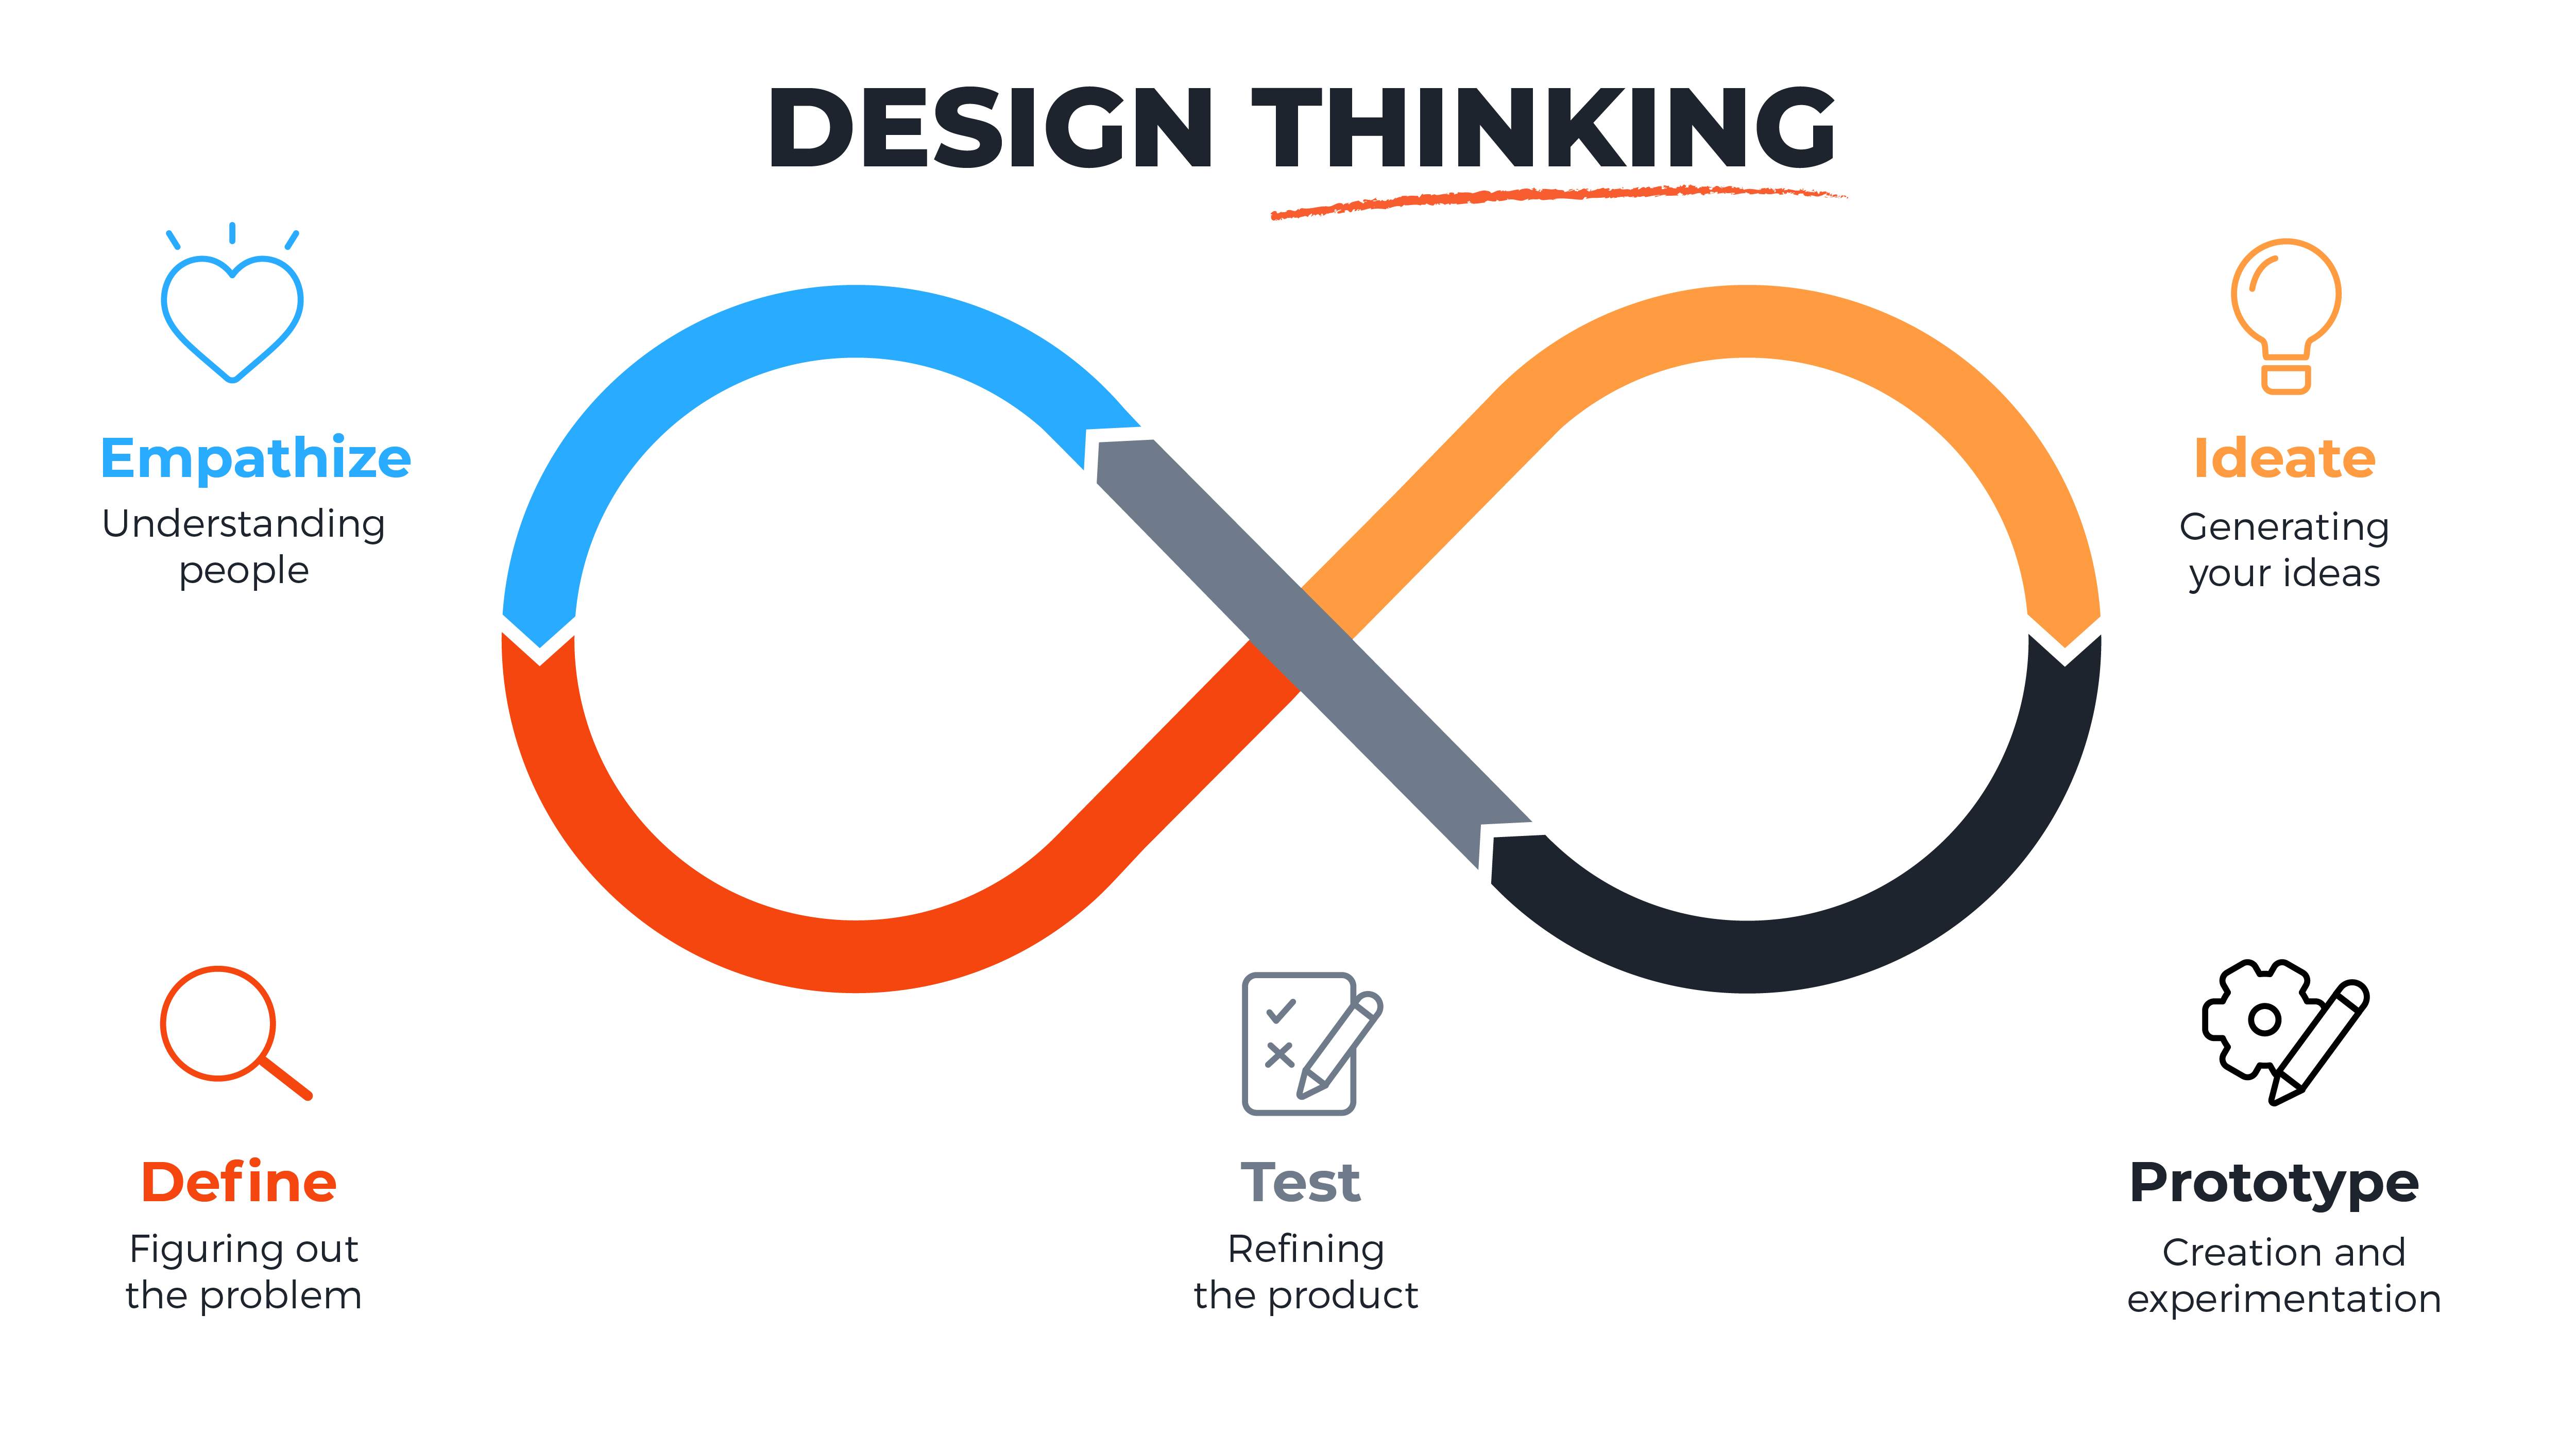
\includegraphics[width=0.8\textwidth]{img/design-thinking.png}
              \end{center}
              \caption{กระบวนการออกแบบ Design Thinking}
              \label{fig:design-thinking}
          \end{figure}

\end{enumerate}


% \noindent
% where $\omega$ is the frequency of the plasmon, $c$ is the speed of
% light, $\varepsilon_m$ is the dielectric constant of the metal,
% $\varepsilon_i$ is the dielectric constant of neighboring insulator,
% and $\varepsilon_\mathit{air}$ is the dielectric constant of air.

% \section{About using figures in your report}

% % define a command that produces some filler text, the lorem ipsum.
% \newcommand{\loremipsum}{
%   \textit{Lorem ipsum dolor sit amet, consectetur adipisicing elit, sed do
%   eiusmod tempor incididunt ut labore et dolore magna aliqua. Ut enim ad
%   minim veniam, quis nostrud exercitation ullamco laboris nisi ut
%   aliquip ex ea commodo consequat. Duis aute irure dolor in
%   reprehenderit in voluptate velit esse cillum dolore eu fugiat nulla
%   pariatur. Excepteur sint occaecat cupidatat non proident, sunt in
%   culpa qui officia deserunt mollit anim id est laborum.}\par}

% \begin{figure}
%   \centering

%   \fbox{
%      \parbox{.6\textwidth}{\loremipsum}
%   }

%   % To include an image in the figure, say myimage.pdf, you could use
%   % the following code. Look up the documentation for the package
%   % graphicx for more information.
%   % \includegraphics[width=\textwidth]{myimage}

%   \caption[Sample figure]{This figure is a sample containing \gls{lorem ipsum},
%   showing you how you can include figures and glossary in your report.
%   You can specify a shorter caption that will appear in the List of Figures.}
%   \label{fig:sample-figure}
% \end{figure}

% Using \verb.\label. and \verb.\ref. commands allows us to refer to
% figures easily. If we can refer to Figures
% \ref{fig:walrus} and \ref{fig:sample-figure} by name in the {\LaTeX}
% source code, then we will not need to update the code that refers to it
% even if the placement or ordering of the figures changes.

% \loremipsum\loremipsum

% % This code demonstrates how to get a landscape table or figure. It
% % uses the package lscape to turn everything but the page number into
% % landscape orientation. Everything should be included within an
% % \afterpage{ .... } to avoid causing a page break too early.
% \afterpage{
%   \begin{landscape}
%   \begin{table}
%     \caption{Sample landscape table}
%     \label{tab:sample-table}

%     \centering

%     \begin{tabular}{c||c|c}
%         Year & A & B \\
%         \hline\hline
%         1989 & 12 & 23 \\
%         1990 & 4 & 9 \\
%         1991 & 3 & 6 \\
%     \end{tabular}
%   \end{table}
%   \end{landscape}
% }

% \loremipsum\loremipsum\loremipsum

% \section{Overfull hbox}

% When the \verb.semifinal. option is passed to the \verb.cpecmu. document class,
% any line that is longer than the line width, i.e., an overfull hbox, will be
% highlighted with a black solid rule:
% \begin{center}
% \begin{minipage}{2em}
% juxtaposition
% \end{minipage}
% \end{center}

\section{\ifenglish%
      \ifcpe CPE \else ISNE \fi knowledge used, applied, or integrated in this project
  \else%
      ความรู้ตามหลักสูตรซึ่งถูกนำมาใช้หรือบูรณาการในโครงงาน
  \fi
 }

\begin{itemize}
    \item 261207 Basic CPE Lab นําความรู้ทางด้านการพัฒนาเว็บแอพพลิเคชัน เช่น HTML, CSS, Tailwind CSS, JavaScript, TypeScript, Next.js
          และ Node.js มาประยุกต์ใช้ในการพัฒนาเว็บแอพพลิเคชัน ทั้งด้านของ front-end ซึ่งจะแสดงผลของเว็บไซต์ และ back-end ที่จะจัดการการทำงานต่าง ๆ รวมถึงการเชื่อมต่อกับฐานข้อมูล
    \item 261361 Software Engineering การใช้กระบวนการทางวิศวกรรมในการดูแลการผลิต ตั้งแต่การเริ่มเก็บความต้องการ การตั้งเป้าหมายของระบบ การออกแบบ กระบวนการพัฒนา การตรวจสอบ การประเมินผลและทดสอบระบบ
    \item 261346 Database Systems การใช้งานฐานข้อมูล โดยใช้ PostgreSQL ในการจัดการฐานข้อมูล รวมถึงการเชื่อมต่อกับฐานข้อมูล
          และการเขียนคำสั่ง SQL ในการดึงข้อมูลจากฐานข้อมูลและการจัดการข้อมูลในฐานข้อมูล

          % \item 261102 Computer Programming การเขียน ทดสอบ และดูแลซอร์สโค้ดของโปรแกรมคอมพิวเตอร์
          %       ซึ่งซอร์สโค้ดนั้นจะเขียนด้วยภาษาโปรแกรม ขั้นตอนการเขียนโปรแกรมต้องการความรู้ในหลายด้านด้วยกัน
          %       รวมถึงการนํา GitHub มาใช้ในการเขียนโปรแกรม
    \item 261200 Object-Oriented Programming ใช้เป็นพื้นฐานในการเขียนโปรแกรมในการพัฒนาเว็บแอพพลิเคชั่น 
\end{itemize}

% อธิบายถึงความรู้ และแนวทางการนำความรู้ต่างๆ ที่ได้เรียนตามหลักสูตร ซึ่งถูกนำมาใช้ในโครงงาน

% \section{\ifenglish%
%       Extracurricular knowledge used, applied, or integrated in this project
%   \else%
%       ความรู้นอกหลักสูตรซึ่งถูกนำมาใช้หรือบูรณาการในโครงงาน
%   \fi
%  }

% อธิบายถึงความรู้ต่างๆ ที่เรียนรู้ด้วยตนเอง และแนวทางการนำความรู้เหล่านั้นมาใช้ในโครงงาน
